% ======================================= %
% WORKFLOW IN COMPUTATIONAL SCIENCE
% ======================================= %

\section[Work Flow]{Work Flow in Computational Science}

\begin{frame}
\frametitle{\large{Version Control in Academia}}
\begin{enumerate}
\item It Creates Reproducible Research
\item It Helps Train New Group Members
\item It Encourages Collaboration
\item It Encourages Good Code Practices
\end{enumerate}
\end{frame}
\note{}

\begin{frame}
\frametitle{\large{More about reproducible research}}
This is a different topic. Nevertheless, is worth mentioning that Purdue is already taking action in this subject
\begin{itemize}
\item  Purdue University Research Repository (PURR): \url{https://purr.purdue.edu/}
\end{itemize}

In the case of GitHub repositories, we can create DOI using \texttt{zenodo.org}
\begin{itemize}
\item A guide here: \url{https://guides.github.com/activities/citable-code/}
\end{itemize}
\end{frame}
\note{}

\begin{frame}
\frametitle{\large{More about reproducible research}}
\begin{columns}[c]
\column{2in}
A cool example

\emph{\small Silverberg, Jesse L., et al. ``Collective motion of humans in mosh and circle pits at heavy metal concerts." Physical review letters 110.22 (2013): 228701.}

\vspace{5mm}
Repo: \url{https://github.com/mattbierbaum/moshpits}
\column{2in}
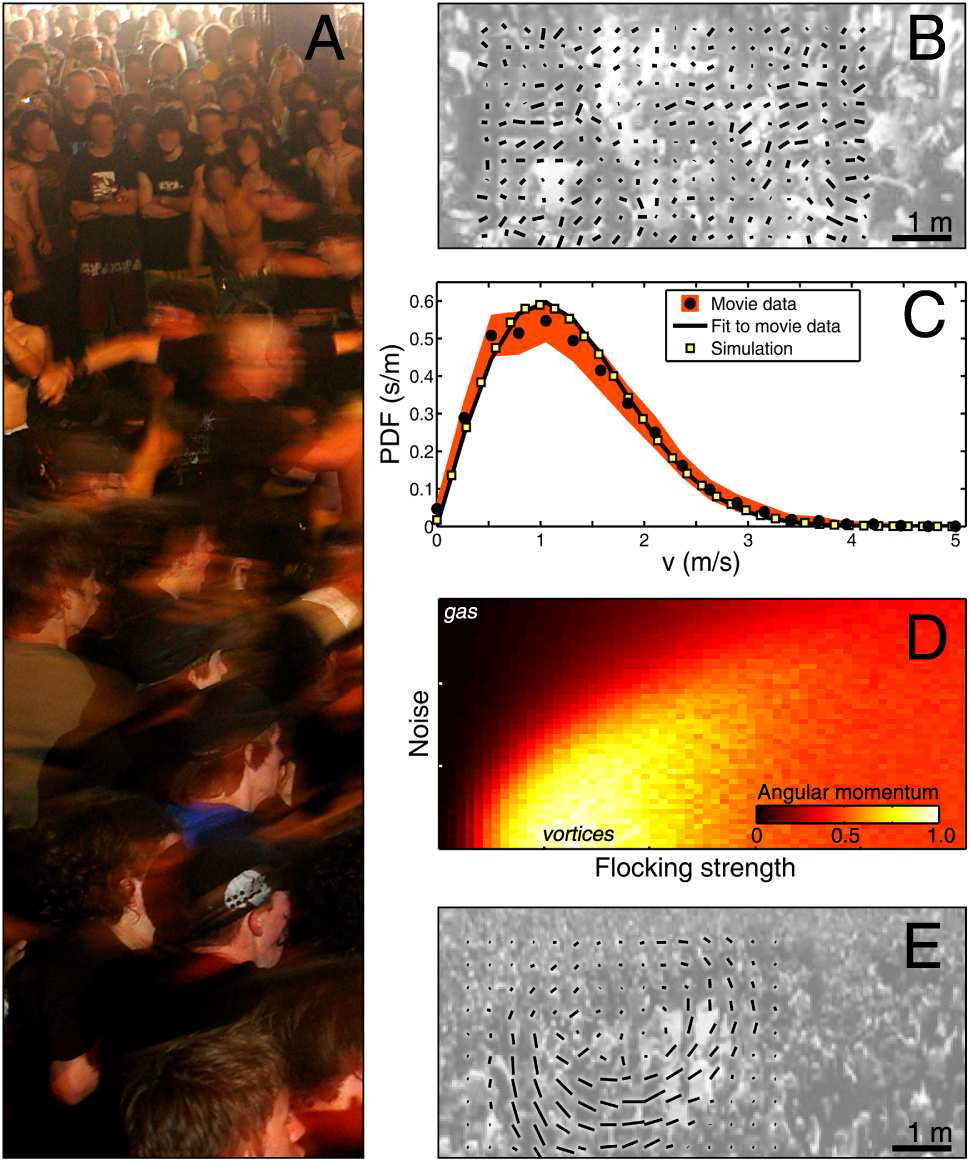
\includegraphics[width=2in]{img/mosh_physics.png} 
\end{columns}




\end{frame}
\note{}

\begin{frame}
\frametitle{\large{Version Control in Academia}}
Some Useful Skills That You Should Learn Are:
\begin{enumerate}
\item Bash
\item Markdown
\end{enumerate}
\end{frame}
\note{}